\documentclass[a4paper,10pt]{article}
\usepackage[utf8x]{inputenc}
\usepackage[pdftex]{graphicx}
\usepackage{hyperref}
\usepackage{array}
\hypersetup{
    colorlinks,
    citecolor=black,
    filecolor=black,
    linkcolor=black,
    urlcolor=black
}
\hypersetup{linktocpage}


%opening
\title{Brief assesment of LD-in-Couch and cumulusRDF}
\author{Teodor Macicas, eXascale, University of Fribourg - Switzerland}

\begin{document}

\maketitle
\clearpage
\clearpage

\begin{abstract}
The target of this document is to provide a brief assesment of both LD-in-Couch (based on CouchDB) and cumulusRDF (based on 
Cassandra) as a storage system for RDF triples. LD-in-Couch easily adapts CouchDB original document based storage back-end to 
allow loading and querying (subject, predicate, object) triples. Our motivation is related to the VeriSign project where this unconventional 
database may be used as a starting point for the local ad-hoc network as well as for the global network. 
As alternative to this we will take into consideration cumulusRDF project based on the well-known and widely used Casandra key-value store. 
It also offers a support for storing and retrieving RDF triples. 
\end{abstract}
\vspace{20 mm}

\section{Introduction}
\subsection{CouchDB}
Note the following information are copied from Wikipedia. I would just add that the last feature seems the most appealing for our One-Laptop-per-Child project.
\paragraph{Document storage}
CouchDB stores data as "documents", as one or more field/value pairs expressed as JSON. Field values can be simple things like strings, numbers, 
or dates; but you can also use ordered lists and associative arrays. Every document in a CouchDB database has a unique id and there is no required document schema.
\paragraph{ACID semantics}
CouchDB provides ACID semantics.It does this by implementing a form of Multi-Version Concurrency Control, meaning that CouchDB can handle a high 
volume of concurrent readers and writers without conflict.
\paragraph{Map/Reduce views and indexes}
The stored data is structured using views. In CouchDB, each view is constructed by a JavaScript function that acts as the Map half of a map/reduce operation. 
The function takes a document and transforms it into a single value which it returns. CouchDB can index views and keep those indexes updated as documents 
are added, removed, or updated.
\paragraph{Distributed Architecture with Replication}
CouchDB was designed with bi-direction replication (or synchronization) and off-line operation in mind. That means multiple replicas can have their own 
copies of the same data, modify it, and then sync those changes at a later time.
\paragraph{REST API}
All items have a unique URI that gets exposed via HTTP. REST uses the HTTP methods POST, GET, PUT and DELETE for the four basic CRUD (Create, Read, 
Update, Delete) operations on all resources.
\paragraph{Eventual consistency}
CouchDB guarantees eventual consistency to be able to provide both availability and partition tolerance.
\paragraph{Built for offline}
CouchDB can replicate to devices (like smartphones) that can go offline and handle data sync for you when the device is back online.

\subsection{LD-in-Couch}
It uses all the features offered by CouchDB plus it makes possible the insertion of RDF triples. It parses the input file, creates (subject, predicate, 
objects) documents as well as back-links if exist. 

\subsection{Cassandra}
Note the following information are copied from Wikipedia.
\paragraph{Decentralized}
Every node in the cluster has the same role. There is no single point of failure. Data is distributed across the cluster (so each node contains different data), 
but there is no master as every node can service any request.
\paragraph{Supports replication and multi data center replication}
Replication strategies are configurable. Cassandra is designed as a distributed system, for deployment of large numbers of nodes across multiple data centers. 
Key features of Cassandra’s distributed architecture are specifically tailored for multiple-data center deployment, for redundancy, for failover and disaster recovery.
\paragraph{Scalability}
Read and write throughput both increase linearly as new machines are added, with no downtime or interruption to applications.
\paragraph{Fault-tolerant}
Data is automatically replicated to multiple nodes for fault-tolerance. Replication across multiple data centers is supported. 
Failed nodes can be replaced with no downtime.
\paragraph{Tunable consistency}
Writes and reads offer a tunable level of consistency, all the way from "writes never fail" to "block for all replicas to be readable", with the quorum level in the middle.
\paragraph{MapReduce support}
Cassandra has Hadoop integration, with MapReduce support. There is support also for Apache Pig and Apache Hive.
\paragraph{Query language}
CQL (Cassandra Query Language) was introduced, an SQL-like alternative to the traditional RPC interface. Language drivers are available for Java (JDBC) and Python (DBAPI2).

\subsection{cumulusRDF}
CumulusRDF is an RDF store on cloud-based architectures. CumulusRDF provides a REST-based API with CRUD operations to manage RDF data. 
This version uses Apache Cassandra as storage backend.

\subsection{The test computer}
Hardware used: 8-core INTEL i7-2600, 8GB main memory, 500GB. \newline
Software: CouchDB 1.2.0, Erlang 5.8.5, Linux OS 3.2.0 kernel version. 

\section{CouchDB - LD-in-Couch}
The following tests were executed on a single machine. However, CouchDB does offer replication, but an auto-sharding mechanism is not available by default. Thus, 
for the moment we restrict the tests on one single machine. Three different data sets were used as it can be seen in the following tables. 

\begin{table}[h]
\centering
\begin{tabular}{|>{\centering}p{2.5cm}|>{\centering}p{2.5cm}|>{\centering}p{2.5cm}|>{\centering}p{2.5cm}|}
    \hline 
    \# triples & \# diff subjects & \# diff predicates  & \# diff objects \tabularnewline
    \hline
    \hline 
    10,693 & 1,745 & 35 & 1,403  \tabularnewline
    \hline 
    97,336 & 15,496 & 35 & 9,193 \tabularnewline
    \hline 
    704,882 & 153,015 & 35 & 87,087 \tabularnewline
    \hline
    4,816,009 & 764,205 & 35 & 433,248 \tabularnewline
    \hline
\end{tabular}
\caption{Data sets}
\label{tab:data_sets}
\end{table}

\subsection{Loading tests}
Three empty databases have been set and for each of them 1 view has been created. This view uses only a map function for emitting document.subject + 
document.graph as key and the entire document as value. Shortly, it permits querying by subject. 
The total loading time can be seen in the following graphs. On y axis the proportion of loaded triples is showed. For instance, 0.6 means that
60\% of them have been already loaded. Intuitively, x axis plots the time in seconds that passed since the beginning of loading.
One note should be made here: the third dataset has been shrinked to 0.7m because the loading time turned out to be too long. 

\paragraph{}
The loading time it may be a bit longer than expected. However, for the first 2 data sets the insertion rate is kept constant across all triples. That is, ~6.7 RDF triples
per second. However, for the bigger dataset it came down to an average of 2.7 RDF triples per second. Taking into considertaion the sizes of input as well as output, we can
assume that often it happened to fill entirely the memory (or different cache layers) and consequently the permanent storage was extensively used. Moreover, the loading process
might also interfered with other higher priority processes of the system. This may explain the time frames with lower insertion rates that are observable on the 
graph as well.

\begin{figure}[h!]
  \centering
  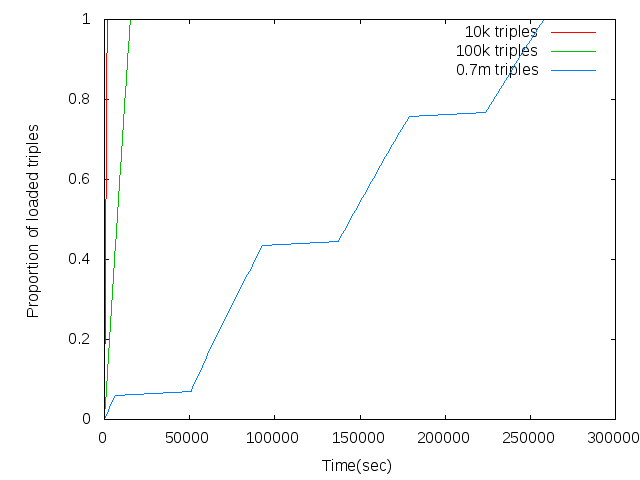
\includegraphics[height=200px]{../couchdb/plots/diff_loading_time.png}
  \caption{Loading time in LD-in-Couch}
  \label{fig:1}
\end{figure}

\paragraph{}
The input file is read line by line and for each it does the following:
\begin{itemize}
 \item create a new document if none exists with the same subject 
 \item if it exists, then update the predicate and object (append) 
 \item query the view to search for a document having as subject the current object 
 \item if found, then create a back link 
\end{itemize}
Internally, couchDB creates 2 B-Trees for each database. One uses document IDs and the other stores document revisions.
If a view is designed, then the view is incrementally updated each time it is used. Thus, in our case, the view gets updated after 
each insertion. However, being an incremental algorithm this has not much impact on the speed. Not to forget is that the view contains
only a map function and it uses the map-reduce paradigm. 
One can argue that the storage size is used by CouchDB unefficiently as for 122k RDF documents it needs 43.2GB. This is partially true 
and a compaction action can be undertaken. 

\begin{table}[h]
\centering
\begin{tabular}{|>{\centering}p{2cm}|>{\centering}p{3cm}|>{\centering}p{2cm}|>{\centering}p{2cm}|>{\centering}p{2cm}|}
    \hline 
    \# triples & \# different documents (unique subjects) & \# document updates & total size  & total loading time\tabularnewline
    \hline
    \hline 
    10,693 & 1,740 & 17,928 & 97.6MB &  26m51s\tabularnewline
    \hline 
    97,336 & 15,493 & 166,161 & 1.9GB & 4h18m13s\tabularnewline
    \hline 
    704,882 & 122,206 & 1,206,010 & 43.2GB & 2days 23h41m32s\tabularnewline
    \hline
\end{tabular}
\caption{Statistics on loading RDF triples using LD-in-Couch}
\label{tab:loading_couch}
\end{table}

\paragraph{}
As CouchDB uses MVCC and is append-only database, each insertion and update create a new document. In case only the last revision of each 
document is intended to be used, one can run a compaction operation which may create another database but storing only the most recent 
versions of each document. As can be seen from the below table, the size dramatically decreased. The duration of this operation 
was in matter of tens of minutes for the biggest data set.

\begin{table}[h]
\centering
\begin{tabular}{|>{\centering}p{2cm}|>{\centering}p{3cm}|>{\centering}p{2cm}|}
    \hline 
    \# triples & total size & size after compaction \tabularnewline
    \hline
    \hline 
    10,693 & 97.6MB & 1.4MB \tabularnewline
    \hline 
    97,336 & 1.9GB & 15.0 MB \tabularnewline
    \hline 
    704,882 & 43.2GB & 116.4MB \tabularnewline
    \hline
\end{tabular}
\caption{Compaction effect on storage size}
\label{tab:compacting_couch}
\end{table}


\subsection{Querying tests}
Five different types of queries have been used as follows: 
\begin{itemize}
 \item select query by subject: given a random existing subject, get the RDF document 
 \item select query by predicate: given a random existing predicate, get the RDF document 
 \item select query by object: given a random existing object, get the RDF document 
 \item select query by id: given a random document ID, get the RDF document 
 \item range query by id: given both start and end key, return all RDF documents (a range can be also provided)
\end{itemize}
The first three types are notated as (s??), (?p?), (??o) in cumulusRDF paper. There are defined also (s?o), (?po), (sp?) which 
were not tested, but they could be implemented as well using Map-Reduce views. 
Finally, the last two query types cannot be executed in cumulusRDF and they may not be so important in this respect.

\begin{figure}[h!]
  \centering
  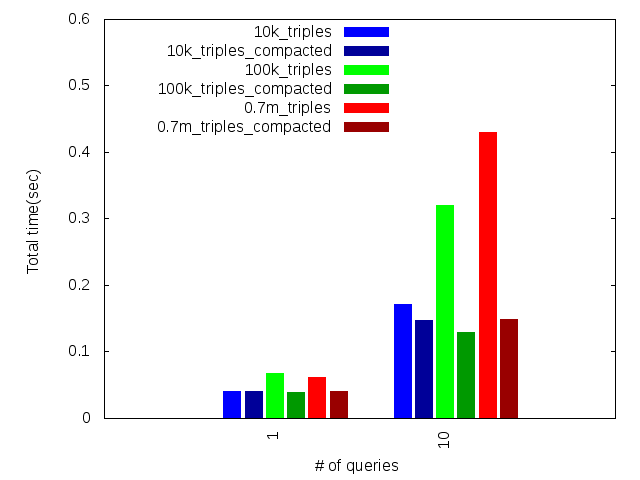
\includegraphics[height=200px]{../couchdb/plots/plot_q_time_1_10.png}
  \caption{Querying by SUBJECT - response time in LD-in-Couch}
  \label{pic:q_subj_1}
\end{figure}
\begin{figure}[h!]
  \centering
  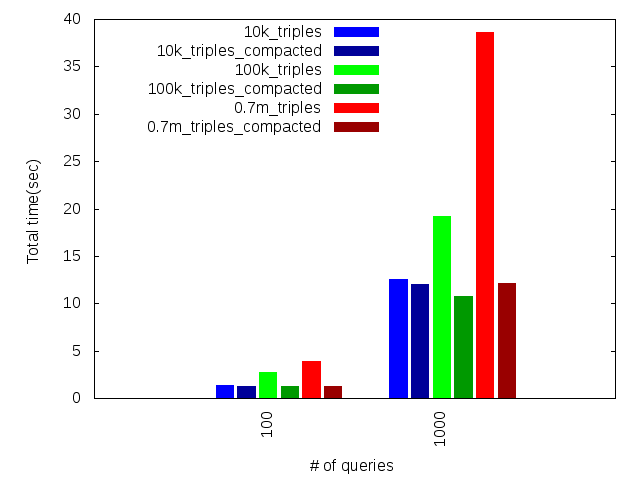
\includegraphics[height=200px]{../couchdb/plots/plot_q_time_10_100.png}
  \caption{Querying by SUBJECT - response time in LD-in-Couch}
  \label{pic:q_subj_2}
\end{figure}
\subsubsection{By subject}
As depicted in pictures~\ref{pic:q_subj_1} and~\ref{pic:q_subj_2}, a series of queries have been run for making the statistics. Every set of queries is run on 
cold cache (hopefully) - couchDB is restarted after every run. Also the views have been updated before running queries. Otherwise, the 
response time of a query might have been influenced by the updates done to the views. 

\paragraph{}
On both graphs there are plotted two different versions of our data sets. One just after loading where all document versions are kept, the 
other called 'compacted' where only the last revision is stored. The latter has been created after loading and represents a different database. 

\paragraph{}
It can be seen that for a single query, the response time is slightly different but it makes no big impact. However, some differences were 
noticed for the 10 queries set. One observation may be that the time remained constant for the compacted versions of databases. 

\paragraph{}
The same trend keeps for bigger query sets. The bigger the database, the slower a query is. However, the retrieving algorithm is O(logN) 
where N is the size of a B-Tree. Since for the 0.7m data set we are talking about a 43GB database, this has a bad impact on the response time 
as well as it may not take advantage of cache locality. Anyhow, the compacted databases still keep an almost constant query time. 

\subsubsection{By predicate}
Another view has been implemented for this purpose. It emits a predicate as a key and the full document as value. 
After creating the views for querying by predicate and by subject, the queries are quite efficient. As in case of Cassandra, 
the search time dominates and it pays off if there are many results. 

\begin{table}[h]
\centering
\begin{tabular}{|>{\centering}p{3cm}|>{\centering}p{3cm}|>{\centering}p{5cm}|}
    \hline 
    query type & query time per result & scale \tabularnewline
    \hline
    \hline 
    by subject & 10\textsuperscript{-2} sec & one \tabularnewline
    \hline 
    by predicate & 10\textsuperscript{-4} sec & tens of thousands \tabularnewline
    \hline 
    by object & 10\textsuperscript{-4} sec & tens of hundreds \tabularnewline
    \hline
\end{tabular}
\caption{Query time per result on 1mil compacted data set}
\label{tab:q_time_per_result_couchdb}
\end{table}

\subsubsection{By object}
Another view has been implemented for this purpose. It emits an object as a key and the full document as value. 
For more information please see Table~\ref{tab:q_time_per_result_couchdb}.

\subsubsection{By ID}
\begin{figure}[h!]
  \centering
  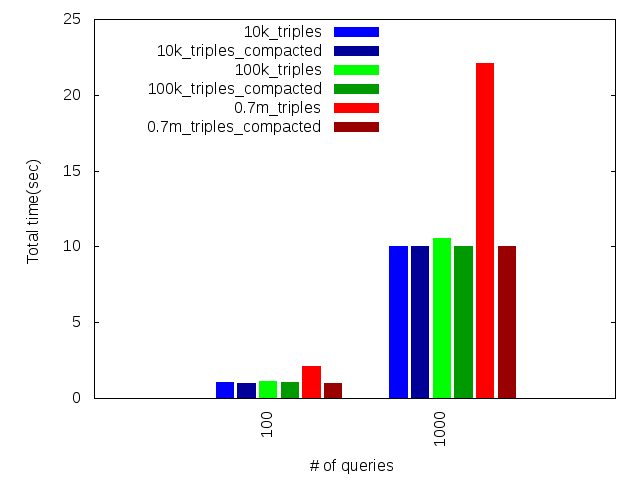
\includegraphics[height=200px]{../couchdb/plots/plot_q_time_id.png}
  \caption{Querying by ID - response time in LD-in-Couch}
\end{figure}
Only the 100 and 1000 query sets have been used as the smaller ones do not give enough hints about how it scales.
As noticed before, the query time still increases with the data size. Again, it keeps almost constant on the compacted versions. This is 
because the actual sizes are way smaller - as it can be seen in Table~\ref{tab:compacting_couch}.

\subsubsection{By ID setting LIMIT}
\begin{figure}[h!]
  \centering
  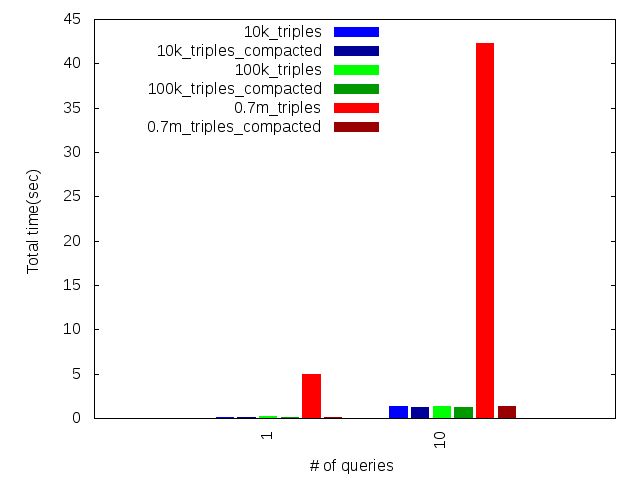
\includegraphics[height=200px]{../couchdb/plots/plot_q_time_id_range.png}
  \caption{Querying by ID LIMIT=1000 - response time in LD-in-Couch}
\end{figure}
\begin{figure}[h!]
  \centering
  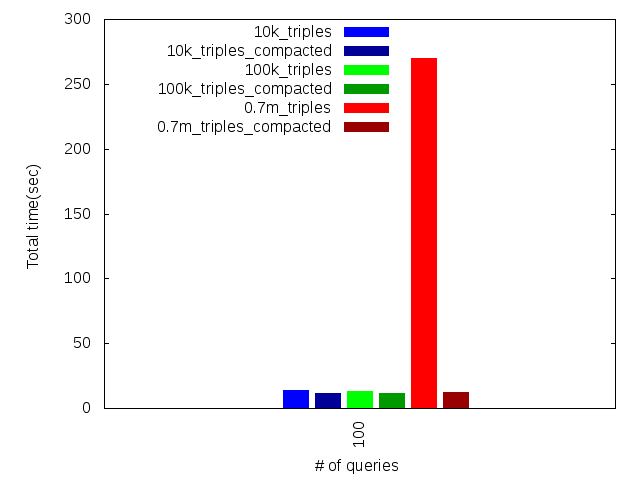
\includegraphics[height=200px]{../couchdb/plots/plot_q_time_id_range_100.png}
  \caption{Querying by ID LIMIT=1000 - response time in LD-in-Couch}
\end{figure}
The difference between a query by ID and this is that a range of documents are returned. As input a start key and a limit is given. Then 
the system finds the document with the given key and traverse the B-Tree leaves (presumably being a B+-tree) and retrieve a maximum of 
'limit' documents (if available). The limit has been set to 1000 documents. 
For this experiment, the data set of 1000 queries has been excluded. Retrieving 1000 times 1000 documents has proved to take quite long time 
especially on the 0.7m non-compacted.
\paragraph{}
Each query returned 1000 documents. Thus, for example, the 100 queries set returned 100,000 documents. 
Somehow expected from previous experiments, the running time is a function of real size on disk (as it uses B-trees). Hence the 
running time for 0.7m data set is quite high. Luckly, the time decreased notably and kept constant for the compacted 
datasets. 

\subsection{Conclusion}
CouchDB is quite a powerful document-oriented database. Being an append-only and using MVCC the storage size could grow fast, but this 
is solved by a compaction operation (storing only most recent versions). The querying time is satisfactory and it's a function (logarithmic) 
of how many documents are stored, including all versions. 
\paragraph{}
The RESTful API proved to be quite easy to use and it integrates well with an web-based application (also the JSON documents' format). 
It's said it has been built to be used offline (even though not tested yet) and this is may be a strong reason to use this system for 
our One-Laptop-per-Child project. 

\section{Cassandra - cumulusRDF}
The following tests were executed on a single machine. However, Cassandra does definitely offer replication and it's able to distribute the tasks.
But for the moment we restrict the tests on one single machine. One reason is to have the same case as we had for CouchDB.

\subsection{Loading tests}
Three different keyspaces have been used and the bulk-loading feature of Cassandra. We measured the clock time as well as the storage size
needed on disk. 
\begin{figure}[h!]
  \centering
  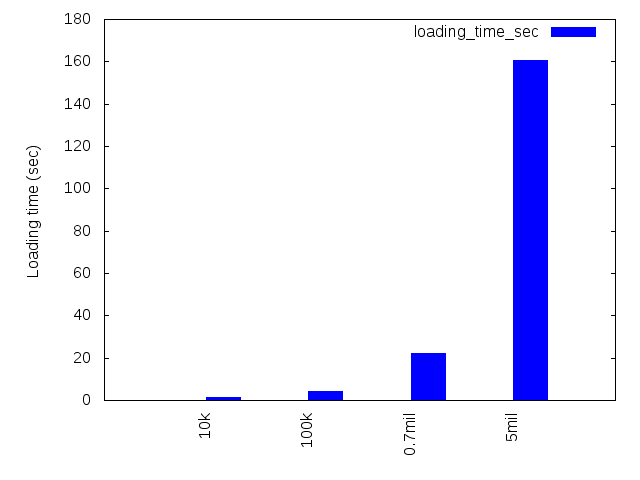
\includegraphics[height=200px]{../cassandra/plots/loading_time.png}
  \caption{Loading time in Cassandra using different data sets}
\end{figure}
Loading time in Cassandra is notably lower than in CouchDB. Actually, it is three orders of magnitude lower in case of ~1mil triples data set. 
This is due to the bulk-loading feature and that Cassandra does not have to update any view every insertion is done. 
Hence it was possible to use another data set with almost 5milion triples.

\begin{table}[h]
\centering
\begin{tabular}{|>{\centering}p{3cm}|>{\centering}p{3cm}|}
    \hline 
    \# triples & total size on disk \tabularnewline
    \hline
    \hline 
    10,693 & 1.5MB \tabularnewline
    \hline 
    97,336 & 7.8MB \tabularnewline
    \hline 
    704,882 & 56MB \tabularnewline
    \hline
    4,816,009 & 449MB \tabularnewline
    \hline
\end{tabular}
\caption{Cassandra storage size on disk}
\label{tab:cassandra_storage_size}
\end{table}
It definitely has a lower footprint on the disk than CouchDB - the compacted versions. Of course, keeping all versions of documents is a 
tradeoff on disk space which is undertaken by CouchDB, but not key-value store of Cassandra. 

\subsection{Querying tests}
Three different types of queries have been used as follows: 
\begin{itemize}
 \item select query by subject: given a random existing subject, get the RDF document (s??) 
 \item select query by predicate: given a random existing predicate, get the RDF document (?p?) 
 \item select query by object: given a random existing object, get the RDF document (??o) 
\end{itemize}

No queries based on ID can be run on Cassandra. However, range queries can be run, but this remains as future task right now. 
Also queries given two parameters are possible. For example, giving subject + object and returning all triples that match both subject 
and object with the input parameters.

\subsubsection{By subject}
\begin{figure}[h!]
  \centering
  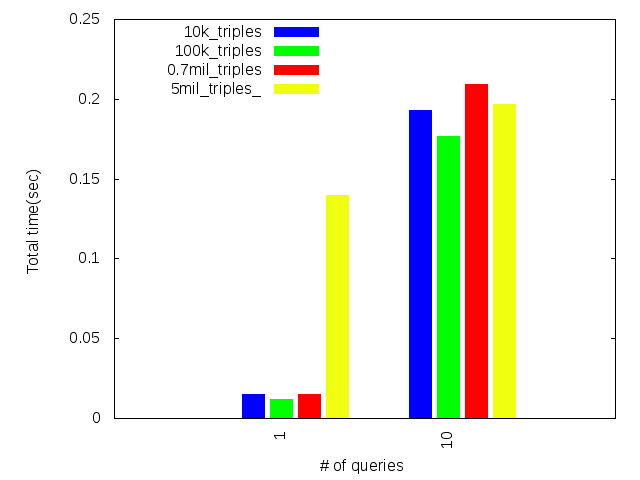
\includegraphics[height=200px]{../cassandra/plots/plot_q_time_by_subj_1_10.png}
  \caption{Querying by SUBJECT - response time in cumulusRDF}
  \label{fig:query_subject_1}
\end{figure}
\begin{figure}[h!]
  \centering
  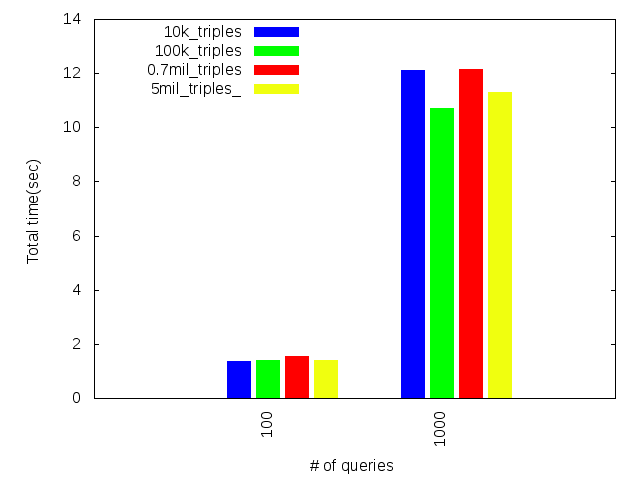
\includegraphics[height=200px]{../cassandra/plots/plot_q_time_by_subj_100_1000.png}
  \caption{Querying by SUBJECT - response time in cumulusRDF}
  \label{fig:query_subject_2}
\end{figure}
One good observations is worth regarding pictures~\ref{fig:query_subject_1} and~\ref{fig:query_subject_2}.
At least in our experiments, the query time remained constant under different data sizes. 

\subsubsection{By predicate}
Having a look at Table ~\ref{tab:data_sets} we can see that there are quite few different predicates across all the data sets. 
Thus, querying by predicate may take much more time than by subject. However, this is only due to the high number of results (usually 
tens of thousands per query for the big data sets).
\paragraph{}
Then, a fair metric would be the time required to retrieve one result. 
It seems that initially the search time is considerable high and then retrieving the results is way faster and it pays off the initial effort.

\begin{table}[h]
\centering
\begin{tabular}{|>{\centering}p{3cm}|>{\centering}p{3cm}|>{\centering}p{5cm}|}
    \hline 
    query type & query time per result & scale \tabularnewline
    \hline
    \hline 
    by subject & 10\textsuperscript{-3} sec & tens \tabularnewline
    \hline 
    by predicate & 10\textsuperscript{-5} sec & tens of thousands \tabularnewline
    \hline 
    by object & 10\textsuperscript{-4} sec & tens of hundreds \tabularnewline
    \hline
\end{tabular}
\caption{Query time per result on 1mil dataset}
\label{tab:q_time_per_result}
\end{table}

\subsubsection{By object}
Please see Table~\ref{tab:q_time_per_result}.

\section{Conclusions}
Both systems have their advantages, obviously. CouchDB offers a very attracting 'built-for-offline' feature with eventual 
consistency. An offline node can modify data as it were online. Once it has again access to the network it can synchronize and all the burden of 
this process is taken care by the system. Another nice feature is versioning of documents. Compaction can get rid of all 
old versions once the storage may be an issue. \newline
The RESTful API it is easy to be used and it would be convenient to integrate it with an web-based application. Also the JSON document 
representation is a clue that this system was designed for the web. \newline 
However, the loading time of an 1million triples would be somehow a limit on this system. Maybe turning off the versioning or finding a way to 
bulk-load would give us better performance.
\paragraph{}
Cassandra offers way faster loading time (using bulk-loading), but almost the same querying time. It's said it scales and it's fault tolerant due to 
replication. However, it does not offer the 'built-for-offline' feature. I would expect Cassandra to offer better performance on 
a large scale network due to the underlaying DHT. \newline
Another nice feature would be the SPARQL and Sesame as a query processor. 
\paragraph{}


\section{Future tasks} 
\begin{itemize}
 \item assess the two systems using replication and/or sharding with many machines 
 \item test how the conflicts caused by updating the same document by multiple clients is solved (specially by CouchDB)
 \item evaluate the usability offline (specially for CouchDB)
 \item evaluate how the system scales on a distributed environment (notably Cassandra)
 \item and whatever could be related to our One-laptop-per-child project 
\end{itemize}


\clearpage
\end{document}
